\documentclass{standalone}
\author{Quinten Bruynseraede}
\usepackage{tikz}
\usetikzlibrary{shapes}
\title{Tikz grafen}
\begin{document}\pagestyle{empty}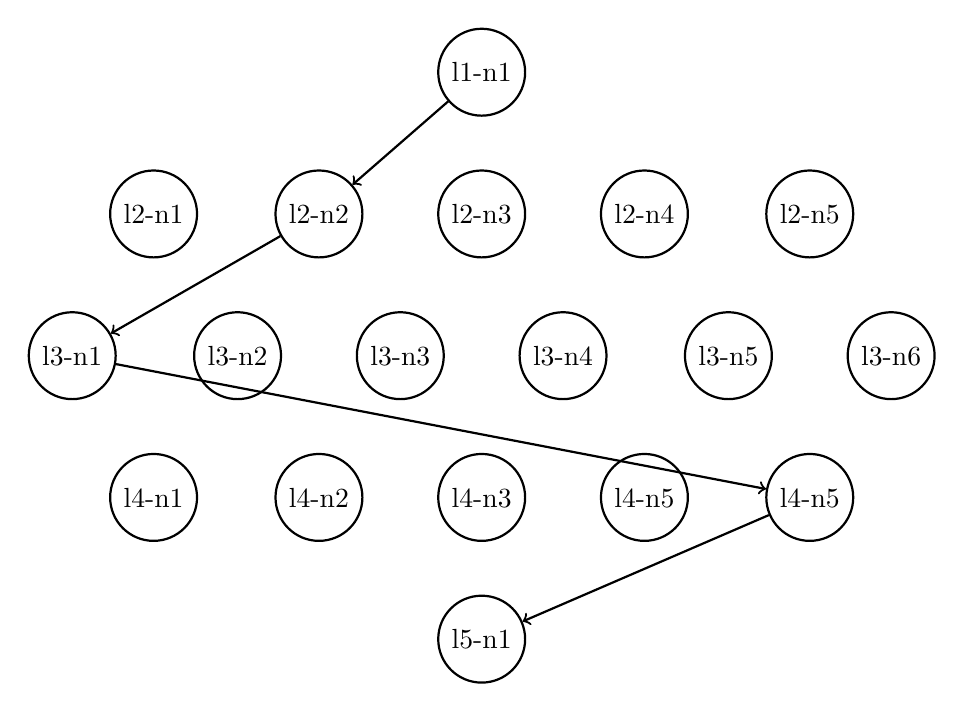
\begin{tikzpicture}\node[shape=circle,draw=black,align=center,line width=0.8pt] (0) at (6.233333333333333,14.866666666666667) {l1-n1};
\node[shape=circle,draw=black,align=center,line width=0.8pt] (1) at (6.233333333333333,13.066666666666666) {l2-n3};
\node[shape=circle,draw=black,align=center,line width=0.8pt] (2) at (4.166666666666667,13.066666666666666) {l2-n2};
\node[shape=circle,draw=black,align=center,line width=0.8pt] (3) at (8.3,13.066666666666666) {l2-n4};
\node[shape=circle,draw=black,align=center,line width=0.8pt] (4) at (10.4,13.066666666666666) {l2-n5};
\node[shape=circle,draw=black,align=center,line width=0.8pt] (5) at (2.066666666666667,13.066666666666666) {l2-n1};
\node[shape=circle,draw=black,align=center,line width=0.8pt] (6) at (5.2,11.266666666666667) {l3-n3};
\node[shape=circle,draw=black,align=center,line width=0.8pt] (7) at (7.266666666666667,11.266666666666667) {l3-n4};
\node[shape=circle,draw=black,align=center,line width=0.8pt] (8) at (9.366666666666667,11.266666666666667) {l3-n5};
\node[shape=circle,draw=black,align=center,line width=0.8pt] (9) at (11.433333333333334,11.266666666666667) {l3-n6};
\node[shape=circle,draw=black,align=center,line width=0.8pt] (10) at (3.1333333333333333,11.266666666666667) {l3-n2};
\node[shape=circle,draw=black,align=center,line width=0.8pt] (11) at (1.0333333333333334,11.266666666666667) {l3-n1};
\node[shape=circle,draw=black,align=center,line width=0.8pt] (12) at (2.066666666666667,9.466666666666667) {l4-n1};
\node[shape=circle,draw=black,align=center,line width=0.8pt] (13) at (4.166666666666667,9.466666666666667) {l4-n2};
\node[shape=circle,draw=black,align=center,line width=0.8pt] (14) at (6.233333333333333,9.466666666666667) {l4-n3};
\node[shape=circle,draw=black,align=center,line width=0.8pt] (15) at (8.3,9.466666666666667) {l4-n5};
\node[shape=circle,draw=black,align=center,line width=0.8pt] (16) at (10.4,9.466666666666667) {l4-n5};
\node[shape=circle,draw=black,align=center,line width=0.8pt] (17) at (6.233333333333333,7.666666666666667) {l5-n1};

\path [->,draw=black,line width=0.8pt] (16) edge node {} (17);
\path [->,draw=black,line width=0.8pt] (0) edge node {} (2);
\path [->,draw=black,line width=0.8pt] (2) edge node {} (11);
\path [->,draw=black,line width=0.8pt] (11) edge node {} (16);
\end{tikzpicture}
\end{document}